\documentclass[11pt]{article}
\usepackage{fullpage} % Required for inserting images
\usepackage{graphicx}
\usepackage[letterpaper,top=2.5cm,bottom=2.5cm,left=2.5cm,right=2.5cm,marginparwidth=2.5cm]{geometry}
\graphicspath{ {./images/} }
\usepackage{wrapfig}

\begin{document}

\title{C Project Final Report (Group 10)}
\author{Adeline [aaw25], Andrea [ayl125], Hanif [hib25], Wen Feng [wfc25]}
\date{19 June 2026}

\maketitle

\section{Part 2 Assembler Structure and Implementation}
\subsection{Modular Design}
\begin{figure}[h]
\centering
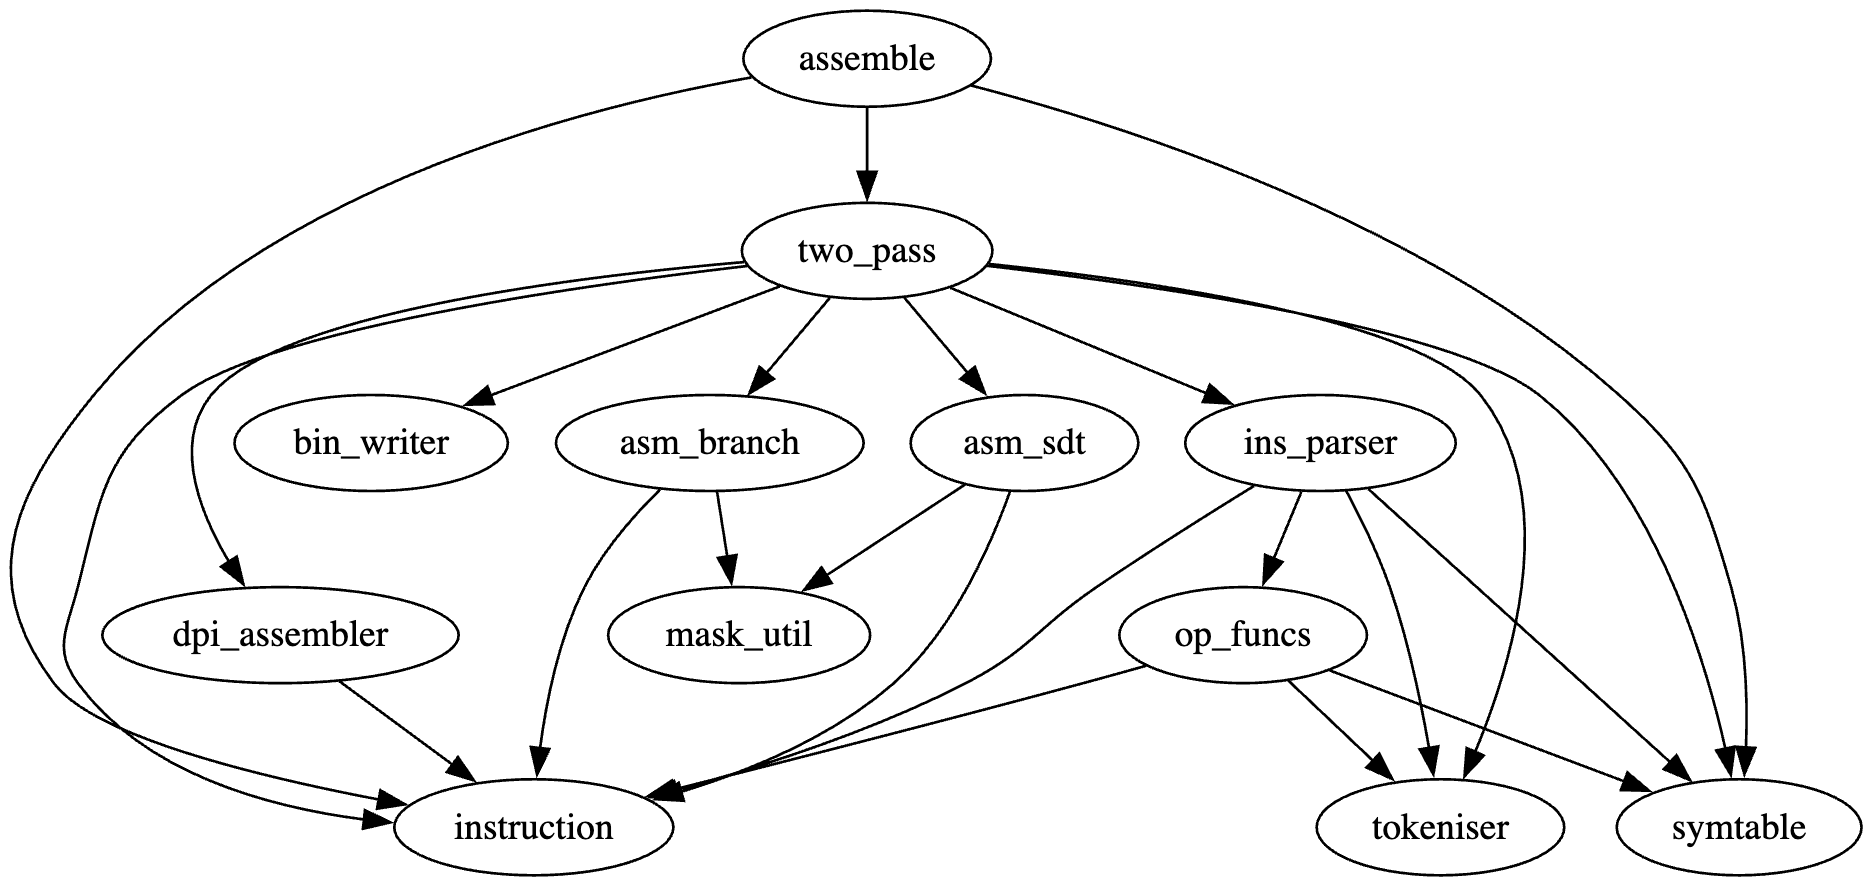
\includegraphics[width=10cm, height = 5cm]{asm-modgraph}
\end{figure}

\subsection{Tokeniser}
The tokeniser was implemented in the tokeniser module. A raw line from the assembly file is turned into a TokenisedLine struct with fields for the label, opcode, an array of operands and the number of operands. If the line contains a colon, it is a label declaration, so only the label is returned, opcode and operands are set to NULL, and the number of operands is set to 0. If not, label is set to NULL and the opcode and operands are extracted. The opcode is extracted using strtok\_r and the operands are extracted by iterating through the rest of the characters and adding a new operand to the array whenever a comma outside a square bracket is encountered. 

\subsection{Symbol Table}
We implemented our symbol table in the symtable module. We used a struct, symkv\_t, to hold a key-value pair of symbol to address, and the symtable struct had fields for an array of key-value pairs, the count of pairs, and the table capacity. We wrote functions to initialise the table, free any allocated memory, insert a new key-value pair, and lookup  the corresponding address in a populated table when given a symbol. 

The array of symkv\_t is dynamic, so the table capacity is increased by an arbitrary number of 100 and memory is reallocated if table capacity is exceeded on insertion of a new key-value pair. The lookup function uses a linear search because we think that the symbol table in the use case of this project is small, so performance will not be impacted significantly. However, if the project were expanded such that the symbol table would become very large, using a hash table to represent the symbol table would make the lookup function much more efficient.

\subsection{Internal Representation of Instruction (shared with emulator)}
We used the same internal representation of an instruction for both the assembler and emulator in instruction.h to reduce code duplication and make debugging easier. The instruction\_t struct has two fields: uint32\_t op0 and a union. op0 defines the instruction type, such as Data Processing (Immediate), Data Processing (Register), Single Data Transfer (Load/Store), Branch, and the .int directive. We also defined a special value for the Halt instruction and a special value EMPTY\_SKIP\_OP0 that will tell the assembler to skip an empty line. (See Section 1.5)

We used a union to hold the structs for each data type and save memory space because each instruction can only be one data type at a time. Each struct contained fields specific to that data type, for example, sf and M for Data Processing (Register). Unions were used within each data type if necessary, such as in the load/store struct to hold 4 structs for the addressing modes of single data transfer, namely unsigned offset, pre/post index, register offset and load literal. The load/store struct had a field called sdt\_mode\_t, an enumerated flag, to ensure safe access to the correct struct in the union.

\subsection{Instruction Parser}
The instruction parser was a combination of the ins\_parser and op\_funcs modules and was responsible for populating the instruction\_t struct. To abstract away the details of how the different operation were parsed, including any sign extension, zero extension or shifts required, the operation functions were all placed in the op\_funcs module. 

An enumerated type op\_t was defined for the types of operations, such as ADD, BCOND, INTDIR and ALIAS. A helper function identifies the op\_t using the opcode of a TokenisedLine. The parse function in ins\_parser uses op\_t to select the corresponding parsing function from an array of pointers to op\_funcs functions, and a helper function is used to parse aliases so the main parse function is kept clean and readable. 

If the opcode is NULL, the parse function returns without populating the union of instruction\_t, but it sets op0 to a special value of EMPTY\_SKIP\_OP0 so the second pass in the two-pass assembly knows to skip the line.

\subsection{Two-pass Assembly}
We decided to implement two-pass assembly as suggested in the spec because we thought it would be more straightforward than one-pass assembly. The first and second passes are written in separate functions to make debugging easier and so the functions can take different parameters. The first pass only takes the assembly input file and a symbol table, while the second pass takes the assembly file, the symbol table, and the output file to write the binary encodings to.
In the first pass, the assembly file is read line-by-line. Each line is tokenised, and if the line is a label declaration, it is added to the symbol table.  
In the second pass, rewind() is used to reset the file pointer  to the start of the assembly file before reading it line-by-line again. The line is tokenised and parsed to populate the instruction\_t struct, which is then passed to the required assembling function to generate the binary encoding. Finally, the binary number is written to the output file.

\subsection{File I/O}
The assembly file reader and binary file writer were initially implemented in the same module, but after completing the other modules and having the second pass function in two\_pass.c write the binary number directly to the output file, we decided to move the assembly file reading out to main() in assemble.c and have the binary file writer in its own module of bin\_writer, to be used by the two\_pass module only.

\subsection{Main assemble.c File}
The assemble.c file uses the modules and functions mentioned above to bring everything together. It opens the assembly file for reading, initialises the symbol table, calls the first and second pass functions, then frees the symbol table and closes the assembly file.

\subsection{Error-checking}
We were careful to prevent buffer overruns by defining maximum line lengths and character lengths, such as for each line of the assembly file, and for the length of the symbol string stored in the symbol table. We printed errors to stderr if the limits were exceeded.

We were also careful to ensure that strings are null-terminated, such as by replacing newline characters with the null terminator when reading lines from the assembly file.

We prevented memory leaks by making sure to free any memory allocated by malloc(), realloc() or strdup(). To avoid double free errors, we checked the opcode and the boolean flag is\_label before freeing the label that used strdup() in instruction. We also checked for memory allocation failures and set pointers to NULL after freeing them to prevent the existence of dangling pointers pointing to deallocated memory. Finally, we confirmed that our program had no memory leaks using valgrind.

Since all the instruction types were defined in the enumerated op\_t type, we could easily check for unknown instruction types and return errors. We also checked for duplicate symbol definitions so the same symbol cannot be added twice to the symbol table.

\section{Part 3 Implementation}
For Part 3, we drove the red LED using GPIO pin 21. We start by
loading the GPIO base address, 0x3f200000, into register w0. Every access is then written as an offset from this base. To make pin 21 an output, we write the value 8 to GPSFSEL2 (offset 0x08), the register that selects the function of pins 20-29. Each pin is governed by a three-bit field, and writing 8 sets pin 21's field to the output configuration while leaving the neighbouring pins unchanged.

With the pin configured as an output, we blink the LED using an
infinite loop made up of two phases separated by delays. To switch the LED on, we set bit 21 and write that value to GPSET0 (offset 0x1c), which drives pin 21 high. We then introduce a delay by zeroing register w10 and incrementing it until it reaches a fixed count, in this case 0x400000 or 4194304, so that the LED stays on long enough to be visible. To switch it off, we write the same bit pattern to GPLCR0 (offset 0x28), driving pin 21 low, followed by an identical delay. Repeatedly cycling through these two phases gives a steady on and off blinking. 


\section{Morse Code Translator (Extension)}

\subsection{Description}
\begin{figure}[h]
    \centering
    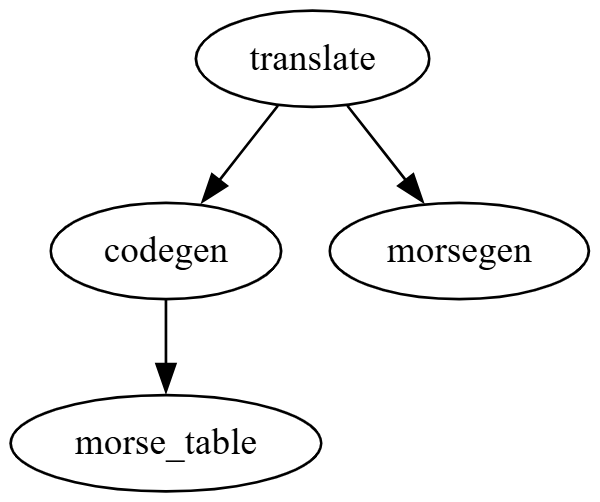
\includegraphics[width=5cm, height=3cm]{ext-modgraph}
\end{figure}
We wanted do something visual with the Raspberry Pi in our extension. With Part 3 fresh in our minds while brainstorming for the extension, we thought of writing code that would take a line of input from a user, translate it into morse code, and write an assembly file for the Raspberry Pi to display the morse code message using the blinking LED.

\subsection{Modular Design}
The extension is split into four modules, each with a single purpose:
\begin{itemize}
    \item translate: the primary file that processes input, manages the workflow, and produces the final assembly output file.
    \item morse\_table: contains the mapping from characters to their Morse representations.
    \item morsegen: produce assembly code for generating delays between each dots, dashes and spaces.
    \item codegen: contains functions to produce the Morse code for a given character using that table.
\end{itemize}

The main process in translate starts with reading the input. The user's line is read with fgets() and copied into the line variable with strcpy(). The output file is then initialised with the assembly preamble. Then, the line is parsed one character at a time. To optimize memory overhead, a helper function first normalises each parsed character by subtracting its base ASCII value ('a' or '0') to generate a zero-based index. This allows the morse\_table to look up characters directly within two compact arrays without needing to allocate a full 256-element ASCII array. This approach removes the redundancy of storing null pointers for unmapped characters while preserving direct indexing. The resulting Morse representation is stored in a variable of type morsecodeline (an array of char). The code is then parsed symbol by symbol. A dot is dispatched to dot\_gen() and a dash to dash\_gen(), each writing the assembly code that blinks the LED for the corresponding duration. Once a character's full Morse sequence has been generated, break\_gen() creates a 1-second delay before the next character is processed. This repeats until the end of the line is reached, after which a halt instruction is written, followed by the definitions of the integer constants referenced by the load-literal instructions. 

\subsection{Challenges}
The primary challenge during the extension's development was managing control flow for the repeated Morse code delay intervals (0.25s for dots, 1s for dashes/breaks and 3s for spaces). Because our assembler strictly enforces unique keys in its symbol table, naively generating identical delay labels across multiple characters caused immediate compilation failures.

We initially explored implementing a subroutine model to share the delay code by manually saving the return address in a register before branching. However, because our implemented subset of AArch64 does not include Branch with Link (bl) or Return (ret) instructions, simulating a call stack required excessive register management, such as maintaining the value of PC to pass return address. Given that our assembler parses linear, inline code highly efficiently, we opted against over engineering a custom call stack. Instead, we dynamically appended an incrementing index to each label during code generation (delay11, delay12).

While manually testing, we encountered inconsistencies in the LED delay timings. Because our assembly relies on instruction-cycle loops rather than a hardware timer, execution overhead gradually caused timing drift. This drift elongated the shorter 'dot' delays, making them visually indistinguishable from 'dashes'. To mitigate this ambiguity, we manually calibrated the delay loops, significantly reducing the cycle count for dots to enforce a strict visual contrast. Given more time, the ideal architectural fix would be to implement deterministic delays by directly polling the Raspberry Pi's hardware System Timer.

\subsection{Testing}
To verify the translator's accuracy, we manually inputted various alphanumeric test strings and cross-referenced the generated output against a standard international Morse code chart. 

\section{Group Reflection}
We communicated primarily through a WhatsApp group chat and online meetings using Google Meet. The group chat was used to update each other about the tasks we were working on. Online meetings were held at the beginning of each part of the project to discuss the implementation and delegation of tasks. Online group calls were also used when we had to work together, for example, when merging and debugging. Our way of communicating was effective and made us aware of the problems each member was facing so we could solve them as a group.

During the first week, one of our group members fell ill, so Part 1 was mostly completed by the other 3 members. To make up for it, she took on more responsibilities in Part 2. The workload for the assembler was split into 8 parts: the binary file writer and assembly file reader, the two-pass assembly, building the symbol table, the tokeniser, the instruction parser, and the three instruction assemblers for data processing, load/ store, and branch. We kept the delegation of tasks fluid since other members were happy to offer help when any one of us had difficulties completing our assigned parts.

An issue our group faced was missing internal deadlines. For Parts 1 and 2, we only completed them two days after our set deadline. More buffer time should be taken into consideration when setting internal deadlines in the future. In addition, we should prioritise writing readable code and document our code as we wrote them to ensure other members understood what we wrote. 

We used online meetings and group calls to plan the direction of the project and discuss ideas. These were very useful in ensuring all group members were on the same page and made our work more efficient. This is something that we would want to keep the same in future group work.

\section{Individual Reflections}

\subsection{Adeline}
I believe I fitted into the group well and contributed well to our work. My strengths and weaknesses were mostly as expected. I communicated clearly with my group members and managed my time well enough to complete all my assigned tasks by the deadline. A weakness I discovered through doing this project was managing stress. I realised that I was always anxious when I was not working on the project and being productive and this negatively affected my mental wellbeing. In the future, I would like to learn better methods to relieve stress and practise them. I would also try to have more buffer time when setting internal deadlines to account for unexpected delays. 

\subsection{Andrea}
I have learned to appreciate the art of clear communication and resolving interpersonal conflict. I had planned to complete most of my work for Part 1 later in the week but fell ill mid-week, significantly shortening the time I was well enough to work. From my previous experiences, I assumed that stating my illness would be enough reassurance for my infrequent updates, but I clearly should have been more direct. Still pacing myself to complete my work by 23:59 on the day of the deadline, I was unaware that my group expected earlier completion, so they assumed I wouldn't finish and completed my part for me. A frustrated message from a group member finally revealed our misaligned expectations. In hindsight, I should have spread my work out more evenly throughout the week. To make up for the extra work my group mates had done in Part 1, I took on more responsibilities in Part 2, completed my tasks as early as possible, and provided more frequent updates. This experience highlighted the importance of proactive communication and the need to account for circumstances beyond my control when managing my time - lessons I will keep in mind for future group projects.

\subsection{Hanif}
Looking back on the project, I've learned a lot about how I work in a team, including what I do well and what I need to improve. The main thing I want to work on is being on time. I was late to most of our meetings, and I know this affected the team, especially since I was the one holding the Raspberry Pi kit. That meant my teammates sometimes had to wait for me before they could start their work. Going forward, I'll make sure to be punctual for every meeting so I don't hold the group back. On the positive side, I think I communicated well with my groupmates. I was always ready to help with any tasks they needed and I was happy to take on extra work too. I really enjoy debugging most of our code and I feel like that was something I brought to the team.

\subsection{Wen Feng}
While working on Part 1, one of our member fell ill and couldn't complete their assigned part. My initial instinct to avoid burdening the group led me to take on an unsustainable share of the codebase, which quickly resulted in burnout. This lead me to realize the importance of consistent communication. I realised that keeping a team aligned requires actively using every tool available. For example, shared project planners, WhatsApp group threads and most importantly highly detailed Git commit logs. Communication is fundamentally simple, yet it is the easiest aspect of a project to neglect when under technical pressure. Ultimately, this experience taught me that a successful project is not just about writing code, it is about writing code as a team.

\end{document}